\section{Supporting Tables for Part I}
\label{app:part1_supporting}

This appendix contains the full Part I evidence material referenced from Deliverables 1--4.

\begin{table}[H]
\centering
\footnotesize
\caption{Interview-based activity model (work-as-imagined / knowledge-as-stated)}
\label{tab:d1_activity_spec}
\rowcolors{3}{black!4}{white}
\begin{tabularx}{\textwidth}{
>{\raggedright\arraybackslash}p{0.07\textwidth}
>{\raggedright\arraybackslash}p{0.25\textwidth}
>{\raggedright\arraybackslash}p{0.11\textwidth}
>{\raggedright\arraybackslash}p{0.08\textwidth}
>{\raggedright\arraybackslash}p{0.14\textwidth}
>{\raggedright\arraybackslash}X
}
\toprule
ID & Activity label & Actor & Order & Expected time & Main tools/resources \\
\midrule
A01 & Stop alarm and orient to time & Participant & 1 & 06:45-06:47 & Smartphone alarm \\
A02 & Drink water & Participant & 2 & 06:47-06:50 & Glass, tap \\
A03 & Toilet and shower & Participant & 3 & 06:50-07:02 & Bathroom, shower \\
A04 & Dress and pack bag & Participant & 4 & 07:02-07:12 & Wardrobe, backpack \\
A05 & Prepare breakfast and coffee & Participant & 5 & 07:12-07:20 & Coffee machine, toaster \\
A06 & Eat breakfast and review schedule & Participant & 6 & 07:20-07:25 & Phone calendar/transport apps \\
A07 & Brush teeth and final grooming & Participant & 7 & 07:25-07:28 & Toothbrush, mirror \\
A08 & Check weather and essentials & Participant & 8 & 07:28-07:30 & Weather app, keys, wallet, ID \\
A09 & Leave apartment for commute & Participant & 9 & 07:30 & Front door, bag \\
\bottomrule
\end{tabularx}
\rowcolors{3}{}{}
\end{table}

\begin{figure}[H]
\centering
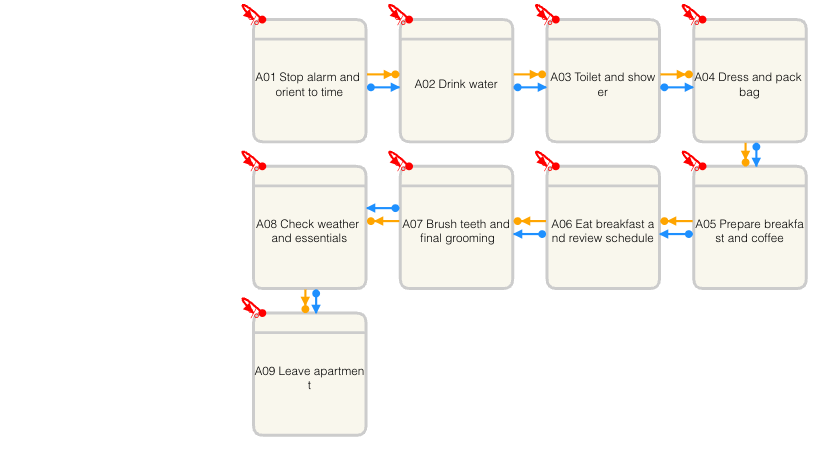
\includegraphics[width=0.95\textwidth]{billeder/dcr_morning_model.png}
\caption{Interview-based DCR graph for the morning routine (A01-A09)}
\label{fig:d1_dcr_graph}
\FigureSource{Own DCR Graph export (February 2026), built from transcript evidence in Appendix~\ref{app:part1_transcript}, Table~\ref{tab:app_transcript_part1} (lines L02-L12, L14-L18, L21-L22).}
\TableNote{Used as baseline \textit{work-as-imagined} model for comparison with observed events in Deliverables 2 and 3.}
\end{figure}

\begin{table}[H]
\centering
\footnotesize
\caption{Observation guide used during Deliverable 2}
\label{tab:d2_observation_guide}
\rowcolors{3}{black!4}{white}
\begin{tabularx}{\textwidth}{
>{\raggedright\arraybackslash}p{0.24\textwidth}
>{\raggedright\arraybackslash}X
>{\raggedright\arraybackslash}p{0.24\textwidth}
}
\toprule
Focus & Observation prompt & Evidence target \\
\midrule
Sequence and boundary & Which event marks start/end, and what is the observed order of actions? & Event IDs, timestamps, sequence notes \\
Tools and artefacts & Which tools/resources are used at each step? & Tool field, context notes \\
Interactions and coordination & Does any interaction with other people occur? & Actor field, coordination notes \\
Deviations from interview baseline & Which actions are skipped, added, reordered, or relabeled relative to A01-A09? & Related activity ID + delta notes \\
Adaptation and recovery & Which workaround or exception handling occurs under time/resource pressure? & Context notes for exception events \\
\bottomrule
\end{tabularx}
\rowcolors{3}{}{}
\TableSource{\textcite{zajac2026methodsknowing} and \textcite{guidehealthinformatics2026ch27}: interview + observation + process-tracing principles adapted to this routine study.}
\TableNote{Field notes were split into descriptive and reflexive notes; only descriptive notes were transcribed into the submitted CSV event log.}
\end{table}

\begin{table}[H]
\centering
\footnotesize
\caption{Observed event-log excerpt (February 20, 2026)}
\label{tab:d2_observed_excerpt}
\rowcolors{3}{black!4}{white}
\begin{tabularx}{\textwidth}{
>{\raggedright\arraybackslash}p{0.08\textwidth}
>{\raggedright\arraybackslash}p{0.16\textwidth}
>{\raggedright\arraybackslash}p{0.20\textwidth}
>{\raggedright\arraybackslash}p{0.12\textwidth}
>{\raggedright\arraybackslash}X
>{\raggedright\arraybackslash}p{0.07\textwidth}
}
\toprule
Event & Timestamp & Event label & Tool & Context note & Ref. \\
\midrule
E01 & 2026-02-20 06:45 & Alarm rings and snooze & Smartphone alarm & One snooze before wake-up. & A01 \\
E03 & 2026-02-20 06:52 & Reply to roommate message & Messaging app & Extra micro-coordination event. & NA \\
E05 & 2026-02-20 06:57 & Toilet and shower & Bathroom & Hygiene block started later than interview expectation. & A03 \\
E07 & 2026-02-20 07:12 & Start coffee and toast & Coffee machine, toaster & Breakfast preparation begins. & A05 \\
E08 & 2026-02-20 07:16 & Switch breakfast to banana & Kitchen & Breakfast adapted due to no bread. & A05 \\
E09 & 2026-02-20 07:18 & Pack bag & Backpack & Packing occurs after breakfast prep starts. & A04 \\
E10 & 2026-02-20 07:21 & Find keys and borrow lock & Keys, messaging app & Workaround to solve missing item. & A08 \\
E14 & 2026-02-20 07:30 & Leave apartment & Front door & End of observed routine boundary. & A09 \\
\bottomrule
\end{tabularx}
\rowcolors{3}{}{}
\end{table}

\begin{table}[H]
\centering
\footnotesize
\caption{Delta sheet between interview model and observed routine}
\label{tab:d3_delta_sheet}
\rowcolors{3}{black!4}{white}
\begin{tabularx}{\textwidth}{
>{\raggedright\arraybackslash}p{0.08\textwidth}
>{\raggedright\arraybackslash}p{0.18\textwidth}
>{\raggedright\arraybackslash}p{0.15\textwidth}
>{\raggedright\arraybackslash}p{0.15\textwidth}
>{\raggedright\arraybackslash}X
>{\raggedright\arraybackslash}p{0.16\textwidth}
}
\toprule
Delta ID & Category & Interview ref. & Observed ref. & Difference description & Implication \\
\midrule
D01 & Missing events & A06 & No direct event & No distinct seated breakfast-and-schedule-review event occurred. & Interview model overstates routine regularity. \\
D02 & Extra events & None in baseline & E03 (06:52) & Short roommate-message coordination appears in observed routine only. & Reveals practical coordination load. \\
D03 & Different order & A04 before A05 & E07 then E09 & Bag packing happened after breakfast preparation started. & Ordering constraints are weaker than stated. \\
D04 & Timing distortions & A03 expected 06:50-07:02 & E05 start 06:57 & Hygiene block shifted later due to wake-up delays. & Time windows in interview are optimistic. \\
D05 & Workarounds/coordination steps & A08 final check & E10 (07:21) & Missing lock triggered ad hoc borrowing via message. & Recovery actions are underrepresented in interview model. \\
D06 & Relabeling/ambiguity & A05/A06 & E08, E13 & ``Breakfast'' changed from sit-down meal to banana plus coffee-to-go. & Label definitions need operational clarity. \\
\bottomrule
\end{tabularx}
\rowcolors{3}{}{}
\end{table}

\section{Supporting Tables and Code for Part II}
\label{app:part2_supporting}

This appendix contains full Part II evidence tables and the custom method code excerpt referenced from Deliverable 6.

\begin{table}[H]
\centering
\footnotesize
\caption{Selected methods from Part 3}
\label{tab:d6_method_selection}
\rowcolors{3}{black!4}{white}
\begin{tabularx}{\textwidth}{
>{\raggedright\arraybackslash}p{0.11\textwidth}
>{\raggedright\arraybackslash}p{0.18\textwidth}
>{\raggedright\arraybackslash}p{0.12\textwidth}
>{\raggedright\arraybackslash}X
}
\toprule
Method & Primary facets & RQ link & Why selected \\
\midrule
M2 & Data, Source, System & RQ1-3 & Baseline completeness check before further interpretation. \\
M6 & Data, Task, Human & RQ1, RQ3 & Captures urgency and temporal representativity in one method. \\
M8 (15 min) & Task, System, Human & RQ2 & Directly tests safety-critical communication conformance. \\
M10 & Data, System, Task & RQ1 & Combines TAT metrics with batch-logging sensitivity. \\
M11 & Human, Task, System & RQ1, RQ3 & Adds workload and actor-distribution context. \\
\bottomrule
\end{tabularx}
\rowcolors{3}{}{}
\end{table}

\begin{table}[H]
\centering
\footnotesize
\caption{Key results and interpretation}
\label{tab:d6_method_results}
\rowcolors{3}{black!4}{white}
\begin{tabularx}{\textwidth}{
>{\raggedright\arraybackslash}p{0.10\textwidth}
>{\raggedright\arraybackslash}p{0.30\textwidth}
>{\raggedright\arraybackslash}X
>{\raggedright\arraybackslash}p{0.15\textwidth}
}
\toprule
Method & Key result & Interpretation (incl. expectation check) & Main facet(s) \\
\midrule
M2 & High missingness in context attributes (e.g., \texttt{study\_uid} 134/150). & As expected; process-flow analysis is possible, but context-dependent inference is limited. & Data, Source \\
M6 & Urgency skew: 15 stat/urgent vs 2 routine; shift imbalance (Day 11, Night 6, Evening 0). & As expected; representativity is uneven, so generalisation should be cautious. & Data, Task, Human \\
M8 & 16 pass, 1 fail (critical case missing communication event). & Worked as intended; even one failed critical case is operationally important for RQ2. & Task, System, Human \\
M10 & Batch logging suspected in 6/17; mean total TAT 147.93 min raw vs 198.50 min clean. & Most surprising output; RQ1 conclusions are highly sensitive to timestamp credibility. & Data, System, Task \\
M11 & Events per role uneven (radiographer 64; resident 7; system actor high concentration). & As expected; workload concentration affects operational and modelling interpretation. & Human, Task, System \\
\bottomrule
\end{tabularx}
\rowcolors{3}{}{}
\end{table}

\begin{table}[H]
\centering
\small
\caption{Facet mapping for Batch Logging Credibility}
\label{tab:d6_custom_facet_mapping}
\rowcolors{3}{black!4}{white}
\begin{tabularx}{\textwidth}{l c X}
\toprule
Facet & Involvement & Justification \\
\midrule
Data & ++ & Timestamp integrity is the direct object of assessment. \\
Source & ++ & Logging practice determines whether entries are real-time or delayed. \\
System & + & Interface/workflow design can incentivise retrospective entry. \\
Task & + & Timeliness-sensitive tasks are directly affected by timestamp quality. \\
Human & + & Workload pressure shapes documentation behavior. \\
\bottomrule
\end{tabularx}
\rowcolors{3}{}{}
\end{table}

\subsection{Custom DQ Assessment Method Code Excerpt}
\label{app:d6_custom_code}

\begin{lstlisting}[style=pycode]
def my_custom_dq_method(df: pd.DataFrame):
    rows = []
    for case_id, cdf in df.groupby('case_id'):
        n = len(cdf)
        u = cdf['event_time'].nunique()
        dup = n - u
        dur = ((cdf['event_time'].max()-cdf['event_time'].min()).total_seconds()/60) if n > 1 else 0
        score = (2 if dup >= 3 else 1 if dup > 0 else 0) + (2 if n >= 5 and dur < 2 else 0) + (1 if (u/n) < 0.5 else 0)
        risk = 'high' if score >= 4 else ('medium' if score >= 2 else 'low')
        rows.append({'case_id': case_id, 'risk_level': risk, 'risk_score': score})
    out = pd.DataFrame(rows)
    flagged = out[out['risk_level'].isin(['high', 'medium'])]
    return {'case_flags': out,
            'summary_metrics': {'total_cases': len(out), 'flagged_case_rate_pct': round(100*len(flagged)/len(out), 2)},
            'examples': flagged.head(3).to_dict('records')}
\end{lstlisting}

\begin{table}[H]
\centering
\footnotesize
\caption{Invisible work not represented explicitly in the event log}
\label{tab:d6_invisible_work}
\rowcolors{3}{black!4}{white}
\begin{tabularx}{\textwidth}{
>{\raggedright\arraybackslash}p{0.23\textwidth}
>{\raggedright\arraybackslash}p{0.18\textwidth}
>{\raggedright\arraybackslash}p{0.13\textwidth}
>{\raggedright\arraybackslash}X
>{\raggedright\arraybackslash}p{0.16\textwidth}
}
\toprule
Activity from diagram & Why not logged? & Facet & Consequence & Capture option \\
\midrule
Radiologist-to-radiologist consultation & Verbal/ad hoc interaction & Human, Task & Understates collaborative interpretation work & Optional peer-consult event \\
Clarification with ordering clinician & Often outside core system & System, Source & Communication-delay attribution may be misleading & Linked communication event \\
Informal reprioritisation/handoff & Local coordination, not formal workflow step & Task, Human & Bottleneck and fairness analyses miss queue management & Priority-adjusted event with reason code \\
\bottomrule
\end{tabularx}
\rowcolors{3}{}{}
\end{table}
